\pdfminorversion=4
\documentclass[aspectratio=169]{beamer}

\mode<presentation>
{
  \usetheme{default}
  \usecolortheme{default}
  \usefonttheme{default}
  \setbeamertemplate{navigation symbols}{}
  \setbeamertemplate{caption}[numbered]
  \setbeamertemplate{footline}[frame number]  % or "page number"
  \setbeamercolor{frametitle}{fg=white}
  \setbeamercolor{footline}{fg=black}
} 

\usepackage[english]{babel}
\usepackage[utf8x]{inputenc}
\usepackage{tikz}
\usepackage{courier}
\usepackage{array}
\usepackage{bold-extra}
\usepackage{minted}
\usepackage[thicklines]{cancel}
\usepackage{fancyvrb}
\usepackage{tabto}

\xdefinecolor{dianablue}{rgb}{0.18,0.24,0.31}
\xdefinecolor{darkblue}{rgb}{0.1,0.1,0.7}
\xdefinecolor{darkgreen}{rgb}{0,0.5,0}
\xdefinecolor{darkgrey}{rgb}{0.35,0.35,0.35}
\xdefinecolor{darkorange}{rgb}{0.8,0.5,0}
\xdefinecolor{darkred}{rgb}{0.7,0,0}
\definecolor{darkgreen}{rgb}{0,0.6,0}
\definecolor{mauve}{rgb}{0.58,0,0.82}

\title[2018-09-07-uchicago-what-am-i-doing]{\huge What am I doing?}
\author{Jim Pivarski}
\institute{Princeton University -- DIANA-HEP}
\date{September 7, 2018}

\usetikzlibrary{shapes.callouts}

\begin{document}

\logo{\pgfputat{\pgfxy(0.11, 7.4)}{\pgfbox[right,base]{\tikz{\filldraw[fill=dianablue, draw=none] (0 cm, 0 cm) rectangle (50 cm, 1 cm);}\mbox{\hspace{-8 cm}\includegraphics[height=1 cm]{princeton-logo-long.png}\includegraphics[height=1 cm]{diana-hep-logo-long.png}}}}}

\begin{frame}
  \titlepage
\end{frame}

\logo{\pgfputat{\pgfxy(0.11, 7.4)}{\pgfbox[right,base]{\tikz{\filldraw[fill=dianablue, draw=none] (0 cm, 0 cm) rectangle (50 cm, 1 cm);}\mbox{\hspace{-8 cm}\includegraphics[height=1 cm]{princeton-logo.png}\includegraphics[height=1 cm]{diana-hep-logo.png}}}}}

% Uncomment these lines for an automatically generated outline.
%\begin{frame}{Outline}
%  \tableofcontents
%\end{frame}

% START START START START START START START START START START START START START

\begin{frame}{}
\Large
\vspace{0.5 cm}
\begin{center}
\textcolor{darkblue}{It's good to give a talk like this because I don't have any \\ ``status report'' meetings to force myself to review.}
\end{center}
\end{frame}

\begin{frame}{End goal: query service}
\large
\vspace{0.5 cm}
I often talk about a ``query service'' to end our reliance on private skims before they become infeasible (HL-LHC).

\begin{center}
\includegraphics[width=0.5\linewidth]{basic-block-diagram.pdf}
\end{center}

\uncover<2->{\textcolor{darkblue}{That's still my end goal, which I use to judge the value of each of my subprojects, but what I'm actually doing is several steps removed from that.}}
\end{frame}

\begin{frame}{Pieces of a query service}
\small
\vspace{0.15 cm}
\begin{columns}
\column{1.1\linewidth}
\begin{itemize}
\item \textcolor{darkblue}{\large Distributed task scheduling:} \uncover<2->{Experimented, have some leads; not actively developing. Igor Mandrichenko's FNAL LDRD project is a promising prototype. Joosep Pata starting on a concept at Caltech. ROOT considering a revamped PROOF. Spark and Dask don't look like realistic options.}

\item \textcolor{darkblue}{\large Query language:} \uncover<3->{Femtocode, my analysis-specialized, zero-runtime-error query language is a working concept, but a new language is not the \underline{\it first} thing we need. I might revive this key ideas in Harrison Prosper and Sezen Sekmen's ``Les Houches Analysis Language'' project.}

\item \textcolor{darkblue}{\large Columnar data storage/management:} \uncover<4->{my intention to collaborate with Carlos Maltzahn's UCSC group petered out. Same with Tanu Malik's database indexing group at DePaul (though indexing is not an \underline{\it early} need). But there's a robust project here at U.Chicago.}

\item \textcolor{darkblue}{\large Columnar ROOT access:} \uncover<5->{originally intended as just a data backend, \textcolor{darkorange}{\bf uproot} is crazy popular. Turning this into a user library diverted some time, but I think it's well spent.}

\item \textcolor{darkblue}{\large Columnar histogramming:} \uncover<6->{intended as an output format for the query service; \textcolor{darkorange}{\bf histbook} was written early to help uproot users do traditional HEP analysis on arrays (to get user feedback).}

\item \textcolor{darkblue}{\large Event/subevent processing engine:} \uncover<7->{columnar manipulation of nested structures is missing from both the data science \underline{\it and} HEP software stacks; opportunity for original CS research.}
\end{itemize}
\end{columns}
\end{frame}

\begin{frame}{}
\Large
\vspace{1 cm}
\begin{center}
\textcolor{darkblue}{Last topic first: columnar manipulation of nested structures}
\end{center}
\end{frame}

\begin{frame}[fragile]{Take inspiration from array programming}
\vspace{0.1 cm}
\hfill \includegraphics[height=2.75 cm]{apl-timeline.pdf}

\vspace{-2.15 cm}
{\bf\large Array programming: Matlab/R/Numpy}

\vspace{0.5 cm}
Expresses regular operations over \\ rectangular data structures in shorthand.

\vspace{0.25 cm}
\begin{itemize}\setlength{\itemsep}{0.15 cm}
\item Multidimensional slices: \tabto{5.5 cm}{\small \mintinline{python}{rgb_pixels[0, 50:100, ::3]}}
\item Elementwise operations: \tabto{5.5 cm}{\small \mintinline{python}{all_pz = all_pt * sinh(all_eta)}}
\item Broadcasting: \tabto{5.5 cm}{\small \mintinline{python}{all_phi - 2*pi}}
\item Masking (list compaction): \tabto{5.5 cm}{\small \mintinline{python}{data[trigger & (pt > 40)]}}
\item Fancy indexing (gather/scatter): \tabto{5.5 cm}{\small \mintinline{python}{all_eta[argsort(all_pt)]}}
\item Row/column commutativity \tabto{5.5 cm}{\small \mintinline{python}{table["column"][7]} (row 7 of column array)}

(hides AoS $\leftrightarrow$ SoA): \tabto{5.5 cm}{\small \mintinline{python}{table[7]["column"]} (field of row tuple 7)}
\item Array reduction: \tabto{5.5 cm}{\small \mintinline{python}{array.sum()}} $\to$ scalar
\end{itemize}
\end{frame}

\begin{frame}[fragile]{Extension to variable-sized, nested structures}
\vspace{0.5 cm}
Logical structure: \tabto{3 cm}{\ttfamily\textcolor{black}{[\textcolor{red}{[}\textcolor{darkblue}{0, 1, 2}], \textcolor{red}{[}], \textcolor{red}{[}\textcolor{darkblue}{3, 4}], \textcolor{red}{[}\textcolor{darkblue}{5, 6, 7, 8, 9}]\textcolor{red}{]}}}

\vspace{0.05 cm}
Offsets:           \tabto{3 cm}{\ttfamily\verb|[|\textcolor{red}{0,}\verb|         |\textcolor{red}{3,}\verb|  |\textcolor{red}{3,}\verb|      |\textcolor{red}{5,}\verb|             |\textcolor{red}{10}\verb|]|}

\vspace{0.05 cm}
Content:           \tabto{3 cm}{\ttfamily\verb|[ |\textcolor{darkblue}{0, 1, 2}\verb|,       |\textcolor{darkblue}{3, 4}\verb|,   |\textcolor{darkblue}{5, 6, 7, 8, 9}\verb|]|}

\vspace{0.05 cm}
Parents:           \tabto{3 cm}{\ttfamily\verb|[ |\textcolor{darkgreen}{0, 0, 0}\verb|        |\textcolor{purple}{2, 2,}\verb|   |\textcolor{darkorange}{3, 3, 3, 3, 3}\verb|]|}

\vspace{0.5 cm}
A ``jagged array'' (content $+$ offsets and/or content $+$ parents) is a basic building block of variable-sized, nested structure.

\begin{itemize}
\item use a jagged array as the content of another jagged array to get {\tt\small list<list<X>>}
\item use a fixed-size rectangular array of dimension {\tt\small N} as content to get {\tt\small list<X[N]>}
\item use a fixed-size rectangular array of dimension {\tt\small M} as offsets to get {\tt\small list<X>[M]}
\end{itemize}

\vspace{0.5 cm}
\uncover<2->{\textcolor{darkblue}{Add columnar tables to the mix and you automatically get jagged tables: \\ e.g.\ arbitrarily many particle records in event records.}}

\end{frame}

\begin{frame}{Array programming can be extended to jagged arrays}
\vspace{0.1 cm}
\begin{columns}
\column{1.05\linewidth}
\begin{itemize}\setlength{\itemsep}{0.15 cm}
\item Multidimensional slices: \tabto{5.5 cm}{\small \mintinline{python}{events["jets"][:, 0]}} $\to$ first jet per event
\item Elementwise operations: \tabto{5.5 cm}{\small \mintinline{python}{jetpt * sinh(jeteta)}} $\to$ \mbox{keep jagged structure\hspace{-1 cm}}
\item Broadcasting: \tabto{5.5 cm}{\small \mintinline{python}{jetphi - metphi}} $\to$ expand {\small \mintinline{python}{metphi}} from

\tabto{5.5 cm}one-per-event to one-per-jet before operation

\item Masking (list compaction): \tabto{5.5 cm}{\small \mintinline{python}{data[trigger]}} $\to$ drop whole events

\tabto{5.5 cm}{\small \mintinline{python}{data[jetpt > 40]}} $\to$ drop jets from events

\item Fancy indexing (gather/scatter): \tabto{5.5 cm}{\small \mintinline{python}{a = argmax(jetpt)}} $\to$ \mbox{\small \mintinline{python}{[[2], [], [1], [4]]}\hspace{-0.5 cm}}

\tabto{5.5 cm}{\small \mintinline{python}{jeteta[a]}} $\to$ \mbox{\small \mintinline{python}{[[3.6], [], [-1.2], [0.4]]}\hspace{-0.5 cm}}

\item Row/column commutativity \tabto{5.5 cm}{\small \mintinline{python}{events["jets"]["pt"][7, 1]}} \mbox{(all the same)\hspace{-0.5 cm}}

(project jagged tables to \tabto{5.5 cm}{\small \mintinline{python}{events["jets"][7]["pt"][1]}}

jagged arrays before indexing): \tabto{5.5 cm}{\small \mintinline{python}{events[7]["jets"]["pt"][1]}}

\tabto{5.5 cm}{\small \mintinline{python}{events["jets"][7, 1]["pt"]}}

\tabto{5.5 cm}{\small \mintinline{python}{events[7]["jets"][1]["pt"]}}

\item Jagged array reduction: \tabto{5.5 cm}{\small \mintinline{python}{jetpt.max()}} $\to$ array of max jet $p_T$ per event
\end{itemize}
\end{columns}
\end{frame}

\begin{frame}[fragile]{Solving physics problems with jagged array programming}
\vspace{0.5 cm}
{\bf Problem:} Compute the $\phi$ difference between each jet and its event's MET.
\small
\begin{minted}{python}
phidiffs = []
for event in dataset:
    event_phidiffs = []
    for jet in event.jets:
        event_phidiffs.append(jet.phi - event.phi)
    phidiffs.append(event_phidiffs)
\end{minted}
\normalsize

\vspace{0.5 cm}
{\bf Jagged array solution:} 
\small
\begin{minted}{python}
# because of extended broadcasting rules
phidiffs = events["jets"]["phi"] - events["MET"]["phi"]
\end{minted}
\end{frame}

\begin{frame}[fragile]{Solving physics problems with jagged array programming}
\vspace{0.5 cm}
{\bf Problem:} Compute mass of all particles from two collections, subjet to a cut.
\small
\begin{minted}{python}
for event in dataset:
    event.leptoquarks = []
    for jet in event.jets:
        for lepton in event.leptons:
            if cut(jet, lepton):
                event.pairs.append(mass(jet, lepton))
\end{minted}
\normalsize

\vspace{0.5 cm}
{\bf Jagged array solution:} 
\small
\begin{minted}{python}
# jagged cross-join makes (jet, lepton) pairs per event
pairs = events["jets"].cross(events["leptons"])

events["leptoquarks"] = mass(pairs[cut(pairs)])
\end{minted}
\end{frame}

\begin{frame}[fragile]{Solving physics problems with jagged array programming}
\vspace{0.5 cm}
{\bf Problem:} Find the ``best'' candidate per event or per subcollection.
\small
\begin{minted}{python}
for event in dataset:
    event.best = []
    for leptoquark in leptoquarks:
        if event.best == [] or \
            quality(leptoquark) > quality(event.best[0]):
                event.best = [leptoquark]
\end{minted}
\normalsize

\vspace{0.5 cm}
{\bf Jagged array solution:} 
\small
\begin{minted}{python}
# jagged argmax makes empty lists [] or singleton lists [N]
argbest = quality(events["leptoquarks"]).argmax()

# jagged fancy indexing transforms [] -> [] and [i] -> [sublist[i]]
events["best"] = events["leptoquarks"][argbest]
\end{minted}
\end{frame}

\begin{frame}{These array programming primitives are vectorizable in hardware}
\vspace{0.25 cm}
\hfill \begin{minipage}{0.2\linewidth}
\begin{center}
\includegraphics[height=2.5 cm]{jaydeep.jpg}

\small Jaydeep Nandi GSoC student
\end{center}
\end{minipage}

\vspace{-3.55 cm}
\includegraphics[width=0.75\linewidth]{hillis-steele-3.pdf}

\vspace{-1.5 cm} Do a parallel prefix scan to compute a cumulative sum in parallel, but use ``parents'' array to mask for same event, then select the last in each event. \vspace{1.5 cm}
\end{frame}

\begin{frame}{These array programming primitives are vectorizable in hardware}
\large
\vspace{0.5 cm}
\begin{columns}
\column{0.5\linewidth}
\mbox{ } \hfill Sum of items in groups \hfill \mbox{ }

\includegraphics[width=\linewidth]{sum_rates_logy.pdf}

\column{0.5\linewidth}
\mbox{ } \hfill Max of items in groups \hfill \mbox{ }

\includegraphics[width=\linewidth]{max_rates_logy.pdf}
\end{columns}

\vspace{0.5 cm}
\normalsize
\textcolor{gray}{cmslpcgpu3.fnal.gov (Xeon Silver 4110 CPU, Tesla P100 GPU)}

\vspace{0.25 cm}
\textcolor{blue}{\small\url{https://github.com/jpivarski/jupyter-performance-studies/blob/master/2018-09-10-jagged-reduction.ipynb}}
\end{frame}

\begin{frame}[fragile]{Like Femtocode, but without the zero-runtime-error guarantee}
\vspace{0.25 cm}
Only four types of arrays are needed to make a reasonably complete typesystem ({\bf PLUR}, as expressive as Protobuf, Avro, Parquet, Arrow, \ldots):
\begin{itemize}
\item {\bf P}rimitive: plain Numpy arrays of numbers, booleans (anything fixed-width)
\item {\bf L}ist: jagged arrays
\item {\bf U}nion: tagged, indexed tuple of arrays
\item {\bf R}ecord: mapping from names to arrays (table)
\end{itemize}

\vspace{0.25 cm}
\begin{uncoverenv}<2->
As well as cross-references ({\bf PLURP} for arbitrary trees, graphs, enum-encoding):
\begin{itemize}
\item {\bf P}ointer: indexed array, possibly with circular references
\end{itemize}
\end{uncoverenv}

\vspace{0.25 cm}
\uncover<3->{Get traditional objects by mixing methods into table rows, tables, and jagged tables.}

\uncover<3->{Get functional programming with syntactic sugar: {\tt\small apply}, {\tt\small filter}, {\tt\small maxby}, \ldots}

\small
\begin{uncoverenv}<4->
\begin{minted}{python}
dimuons      = muons.pairs(same=False).apply(lambda a, b: a + b)
\end{minted}
\end{uncoverenv}
\vspace{-0.35 cm}
\begin{uncoverenv}<5->
\begin{minted}{python}
good         = dimuons.mass().apply(lambda m: (40 < m) & (m < 140))
\end{minted}
\end{uncoverenv}
\vspace{-0.35 cm}
\begin{uncoverenv}<6->
\begin{minted}{python}
leading      = dimuons[good].maxby(lambda z: z.pt())
\end{minted}
\end{uncoverenv}
\vspace{-0.35 cm}
\begin{uncoverenv}<7->
\begin{minted}{python}
boosted_jets = jets.boost(leading.boostvector())    # broadcasted
\end{minted}
\end{uncoverenv}
\end{frame}

\begin{frame}{Working examples in uproot 3: try it out!}
\vspace{0.25 cm}
\textcolor{blue}{\small\url{https://mybinder.org/v2/gh/scikit-hep/uproot/master?filepath=binder\%2Fversion-3-features.ipynb}}

\vspace{0.15 cm}
\includegraphics[width=\linewidth]{tutorial-screenshot.png}
\end{frame}

\begin{frame}{Next topic}
\Large
\vspace{1 cm}
\begin{center}
\includegraphics[width=0.3\linewidth]{uproot-logo.pdf}
\end{center}
\end{frame}

\begin{frame}{uproot is crazy popular}
\vspace{0.5 cm}
Nearly 1~year from version~1.0 to version~3.0.0b2 $\to$ 551 unique downloaders.

\textcolor{gray}{\scriptsize (``Uniqueness'' defined as same country code, OS distribution, version, and kernel; may over- or under-count.)}

\includegraphics[height=4.2 cm]{uproot-pip-vsweek.pdf}
\only<1>{\hfill \includegraphics[height=4.2 cm]{uproot-pip-numdownloads.pdf}}
\only<2-3>{\includegraphics[height=4.2 cm]{uproot-pip-vscountry.pdf}}
\only<2>{\includegraphics[height=4.2 cm]{uproot-pip-vsos.pdf}}
\only<3>{\includegraphics[height=4.2 cm]{uproot-pip-vsoscountry.pdf}}
\end{frame}

\begin{frame}{Pure Python+Numpy has good performance for large baskets}
\vspace{0.5 cm}

\begin{columns}
\column{0.55\linewidth}
\mbox{ } \hfill Speedup relative to C++ ROOT (3$\times$) \hfill \mbox{ }

\includegraphics[width=\linewidth]{root-none-muon.png}

\column{0.55\linewidth}
\mbox{ } \hfill Speedup relative to root\_numpy (30$\times$) \hfill \mbox{ }

\includegraphics[width=\linewidth]{rootnumpy-none-muon.png}
\end{columns}

\vspace{0.5 cm}
The key is that uproot does {\it less work---} it only delivers arrays (jagged arrays, above). It does not create event objects.
\end{frame}

\begin{frame}{That's why I've been focusing so much on manipulating arrays}
\vspace{0.3 cm}
\begin{columns}
\column{1.15\linewidth}
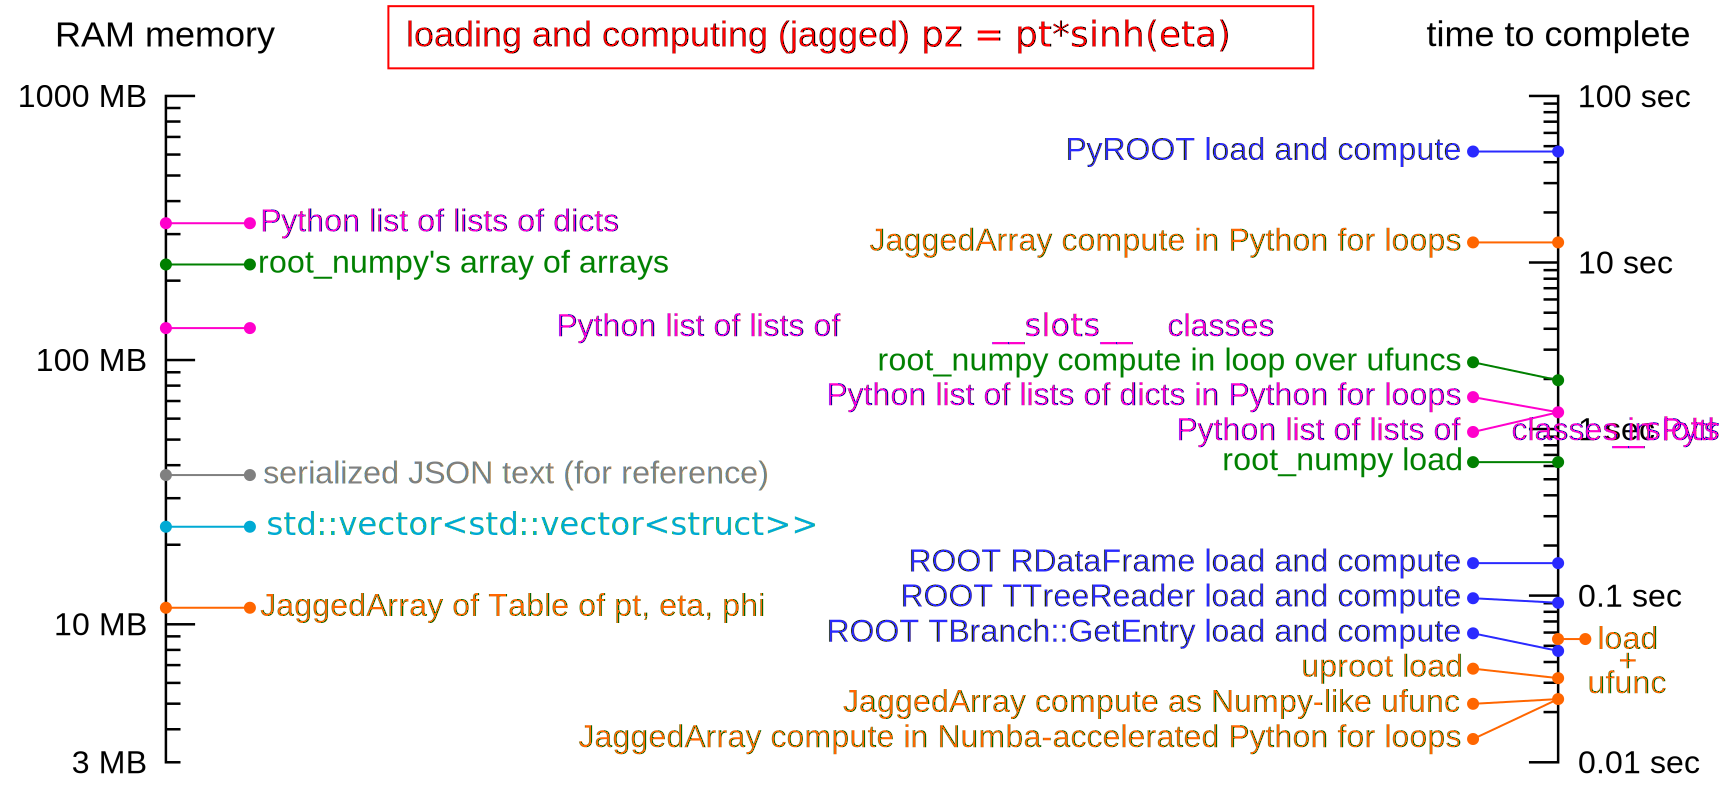
\includegraphics[width=\linewidth]{logscales.pdf}
\end{columns}
\end{frame}

\begin{frame}{Next topic}
\large
\vspace{1 cm}
\begin{center}
\includegraphics[width=0.4\linewidth]{histbook-logo.pdf}
\end{center}
\end{frame}

\begin{frame}{``Reduced query output'' object rich enough for offline analysis}
\Large
\begin{center}
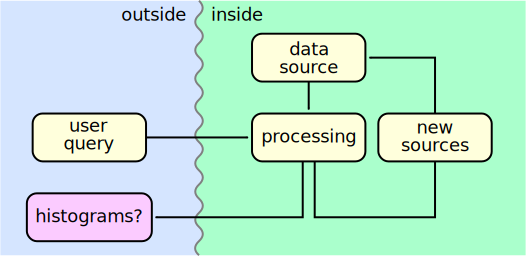
\includegraphics[width=0.5\linewidth]{basic-block-diagram-2.pdf}
\end{center}

\begin{itemize}
\item Must be array-ready: 
\item Should be able to delay plotting decisions: multidimensional block of bins for later slicing and projecting.
\item 


\end{itemize}
\end{frame}






\end{document}
